\documentclass[11pt,a4paper]{article}

\usepackage[applemac]{inputenc}
\usepackage{latexsym}
\usepackage{graphicx}
\usepackage[francais]{babel}
\usepackage{amsmath,amssymb}
\usepackage{pstricks,pst-plot}
\usepackage{calc}
\usepackage{multicol}
\usepackage{fancyhdr}
\usepackage{lastpage}
\usepackage[T1]{fontenc}
\usepackage{stmaryrd}
\pagestyle{plain}



\title{Programming Assignment 1 \\ From planning to reinforcement learning}
\author{Mathurin \textsc{Massias} \and Cl�ment \textsc{Nicolle}}
\date{\today} 

\begin{document}
\maketitle

\section{Simulated trajectories and estimation of value function}
\hspace{-6mm}\textbf{Question 1}: At a given week, the shop owner has what he had last week, plus what he received (and this sum cannot be greater than the maximum he can stock), minus what he sold, and he cannot sell more than he has, so this difference cannot be negative.
\\The reward at a given week is equal to: minus the fix cost of delivery (if he orders), minus the cost of his command, minus maintenance cost, plus the sales.

\section{Policy evaluation}
\hspace{-6mm}We wrote three functions:
\\- pol\_eval\_1(pi, P, R, gamma) computes V using the matricial equation $V^{\pi} = R + \gamma PV^{\pi}$, which leads to $V^{\pi} = (I - \gamma P)^{-1} R$. In these equations $R$ and $P$ are not the general 2D and 3D matrices, but the 1D and 2D matrices associated to a given policy $\pi$ = $R = R(x, \pi(x))$ and $P = P(x, y, \pi(x))$.
\\- pol\_eval\_2(MCn,n,V0,pi,D,M,K,h,c,pr,gamma) computes an estimation of $V$ using MCn Monte-Carlo simulation for each coordinate. It is slow, converges slowly (in $\sqrt{n}$ by LLN), and does not provide an exact value of $V^{\pi}$.
\\- pol\_eval\_3(pi, P, R ,gamma, n\_it) compute $V^{\pi}$ using n\_it iterations of the Bellman operator. Same here, $P$ and $R$ are adapted to the peculiar policy $\pi$.


\section{Value iteration, policy iteration}
\hspace{-6mm}For real code see VI.m and PI.m files.
\\Pseudo code for policy iteration :
\begin{verbatim}
start at any pi = pi_0
for i = 1, ..., N_it
    evaluate V_pi
    compute Q(x,a) = R(x,a) + gamma * sum_y P(x,y,a) V_pi (y)
    set pi(x) =arg max Q(x,a) (over a) (improvment)
end for
return pi
\end{verbatim}
%
Pseudo code for value iteration:
\begin{verbatim}
start at any V = V_0
for i = 1, ..., N_it
    compute Q(x,a) = R(x,a) + gamma * sum_y P(x,y,a) V(y)
    set V = max Q(x,a) (over a) (improvment)
end for
return pi(x) = arg max Q(x,a) (over a)
\end{verbatim}
%
Both give $\pi^* = (10, 9, 8, 7, 0, ...., 0)^T$. So there is sort of a "threshold" : whenever stocks goes under 4 units, the owner must refill to get 10 units. Otherwise he does nothing. It is a balance between the risk of being short on product and missing sales, and the cost of maintenance + the cost of order.
%
\begin{figure}[!htbp]
\centering
\noindent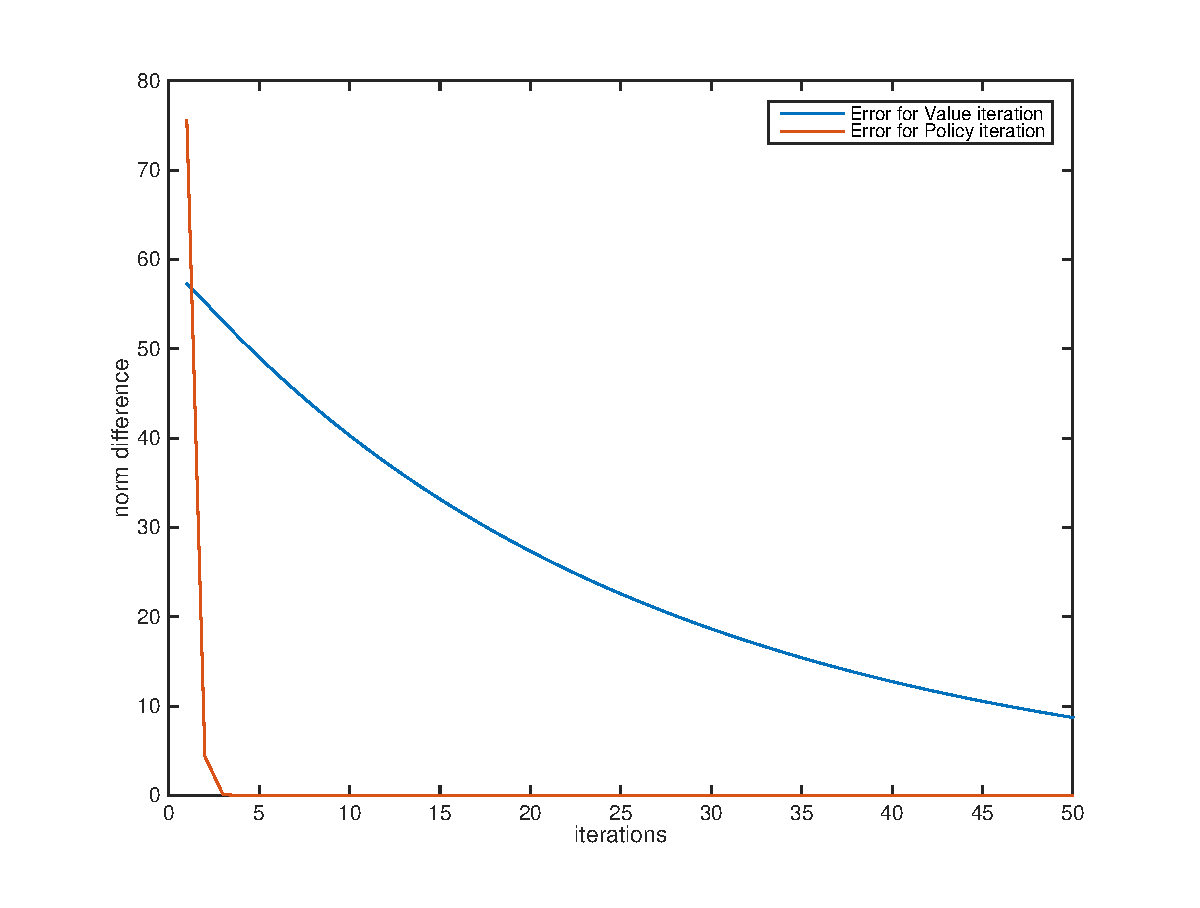
\includegraphics[scale=0.6]{Convergence_VIPI.eps}
\caption{Convergence after $k$ iterations of PI and VI algorithms}
\end{figure}



\end{document}